%%%%%%%%%%%%%%%%%%%%%%%%%%%%%%%%%%%%%%%%%%%%%%%%%%%%%%%%%%%%%%%%%%%%%%
\begin{frame}[fragile]\frametitle{}
\begin{center}
{\Large Binary Search}
\end{center}

\end{frame}

%%%%%%%%%%%%%%%%%%%%%%%%%%%%%%%%%%%%%%%%%%%%%%%%%%%%%%%%%%%%%%%%%%%%%%
\begin{frame}
	\frametitle{Searching in a sorted list}
	
	\begin{columns}
		\column{0.505\textwidth}
	\begin{center}
		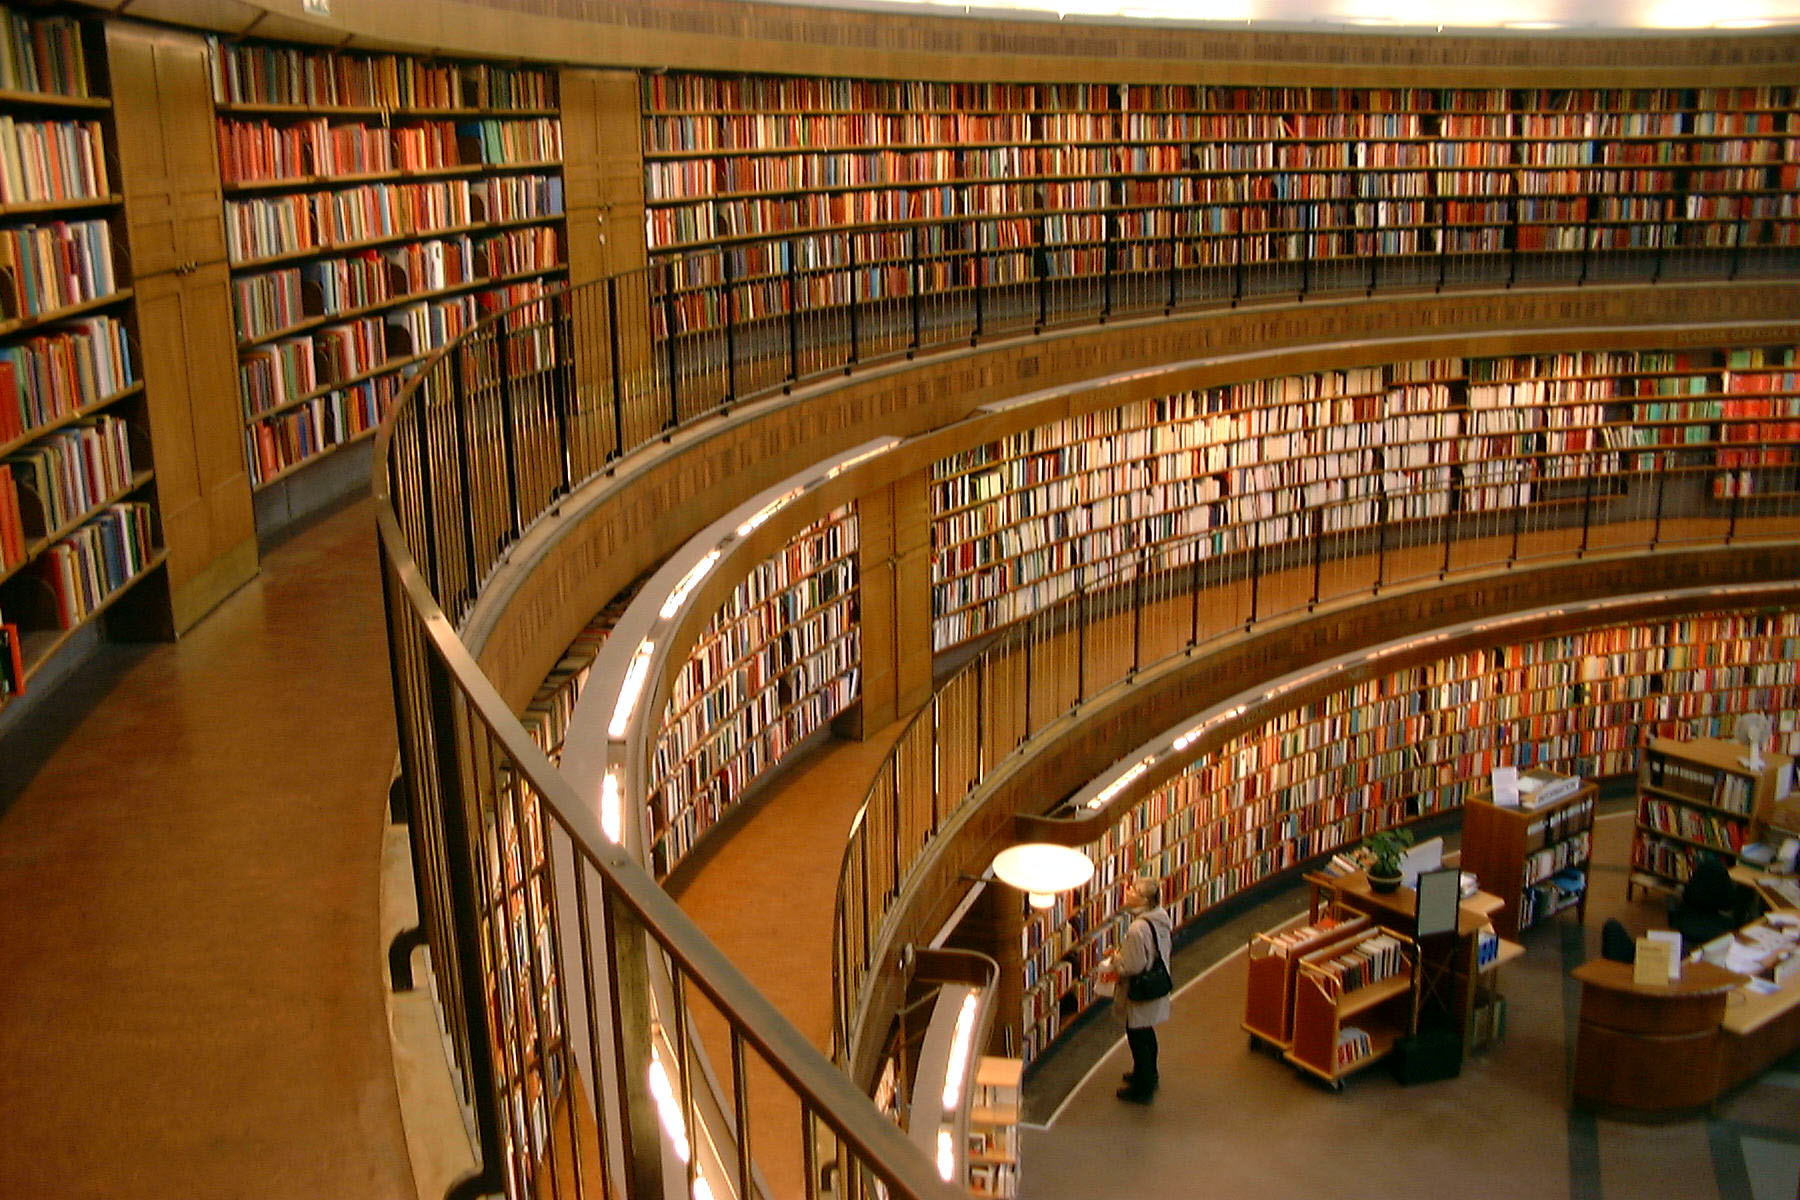
\includegraphics[width=0.9\textwidth]{images/library.jpg}\\
		\hspace*{15pt}\hbox{\scriptsize Image By:\thinspace{\itshape Marcus Hansson}}
		% https://commons.wikimedia.org/wiki/File:Interior_view_of_Stockholm_Public_Library.jpg
	\end{center}
		\column{0.455\textwidth}
			\begin{itemize}
			\item How do you look for books in a library? Say for instance you look for ``To kill a mockingbird'' by Harper Lee.
				\item You see ``Split second'' by David Baldacci and you need to look further down the shelf.
					
				\item You see ``The Amber Spyglass'' by Philip Pullman and you need to go back\dots
					
				\item Let's formalise that idea!
			\end{itemize}
	\end{columns}
\end{frame}

%%%%%%%%%%%%%%%%%%%%%%%%%%%%%%%%%%%%%%%%%%%%%%%%%%%%%%%%%%%%%%%%%%%%%%
\begin{frame}
	\frametitle{Déjà Vu all over again?}
	
			A recursive function is a function that calls itself.
		
		\begin{columns}
			\column{0.455\textwidth}
				For instance for Fibonacci:
				\begin{align*}
					F(1) &= 1 \\
					F(2) &= 1 \\
					F(n) &= F(n-1) + F(n-2) \text{ if $n > 2$}\\
				\end{align*}
			\column{0.455\textwidth}
			
		\lstinputlisting{src/fib.py}
				
		\end{columns}
\end{frame}

%%%%%%%%%%%%%%%%%%%%%%%%%%%%%%%%%%%%%%%%%%%%%%%%%%%%%%%%%%%%%%%%%%%%%%
\begin{frame}
	\frametitle{Binary Search}

			\begin{itemize}
			\item Given a sorted list $L$, determine if it contains an item with value $v$.
			\item Example: Sorted names:
			\begin{itemize}
			\item \texttt{L = [Angelova, Chong, Hugtenburg, Sijm, van den Akker]}
			\item Does it contain \texttt{Sijm}?
			\item Answer: Yes!
			\end{itemize}

			\item \alert{But how do we get there?}
			\item Remember that \texttt{in} from Python takes $\Theta(n)$ time. We want to improve on that!
		\end{itemize}	
\end{frame}

%%%%%%%%%%%%%%%%%%%%%%%%%%%%%%%%%%%%%%%%%%%%%%%%%%%%%%%%%%%%%%%%%%%%%%
\begin{frame}
	\frametitle{Binary search}
	
		Let's build this algorithm:
		
			\begin{columns}[t]
					
				\column{0.455\textwidth}
		\begin{itemize}
\item If the list is empty, return false
		\item Otherwise\dots Take the middle element of the list with index \texttt{m}, with value $x$.
		\item If $x = v$, return true.
		
		\item If $x > v$, return binary search in \texttt{L[:m]}.{start looking in the left{\_\_\_} side of the list.}
		\item If $x < v$, return binary search in \texttt{L[m+1:]}.{start looking in the right{\_\_\_} side of the list.}
		\end{itemize}
				\column{0.605\textwidth}

			\lstinputlisting{src/binary-search.py}	

			\end{columns}


\end{frame}

%%%%%%%%%%%%%%%%%%%%%%%%%%%%%%%%%%%%%%%%%%%%%%%%%%%%%%%%%%%%%%%%%%%%%%
\begin{frame}
	\frametitle{Binary search}

Filling in the blanks:

				What should we put on the blanks?
				
				\begin{itemize}
					\item `left' on line 3 and `left' on line 4. 
					\item `left' on line 3 and `right' on line 4. 
					\item `right' on line 3 and `left' on line 4. 
					\item `right' on line 3 and `right' on line 4. 
					\item I don't know.
				\end{itemize}	

Pseudocode:
				The above is what some might call \textit{pseudocode}. A natural language description of our program.			

				But just on the board, rather than in the slides.

\end{frame}

%%%%%%%%%%%%%%%%%%%%%%%%%%%%%%%%%%%%%%%%%%%%%%%%%%%%%%%%%%%%%%%%%%%%%%
\begin{frame}
	\frametitle{So how well does this do?}

Reminder: 			Our time to beat is the Python built-in \texttt{in} operator that requires $\Theta(n)$ time!

		\begin{columns}
			\column{0.605\textwidth}
				\lstinputlisting{src/binary-search.py}	
			\column{0.405\textwidth}
			
				\begin{itemize}
					\item What is the runtime of this function? 
					\item Try to formulate a recursive $T(n)$, where $n$ is \texttt{len(L)}.
					\item $T(0) = c_0$ for lines 5 and 6.
					\item $T(n) = T(\lfloor n/2 \rfloor) + c_1 + c_2n$ for lines 8 through 15.
			\end{itemize}
		\end{columns}
\end{frame}

%%%%%%%%%%%%%%%%%%%%%%%%%%%%%%%%%%%%%%%%%%%%%%%%%%%%%%%%%%%%%%%%%%%%%%
\begin{frame}
	\frametitle{So how well does this do? In terms of space $S(n)$}

		\begin{columns}
			\column{0.605\textwidth}
			\lstinputlisting{src/binary-search.py}	
			\column{0.405\textwidth}
				\begin{itemize}
					\item What is the runtime of this function? 
					\item Try to formulate a recursive $S(n)$, where $n$ is \texttt{len(L)}.
					\item $S(0) = c_0$ for lines 5 and 6.\\
					\item $S(n) = S(\lfloor n/2 \rfloor) + c_1 + c_2n$ for lines 8 through 15.
			\end{itemize}
		\end{columns}
\end{frame}

%%%%%%%%%%%%%%%%%%%%%%%%%%%%%%%%%%%%%%%%%%%%%%%%%%%%%%%%%%%%%%%%%%%%%%
\begin{frame}
	\frametitle{No improvements}
Reminder:
			Our time to beat is the Python built-in \texttt{in} operator that requires $\Theta(n)$ time!

Making it strictly better:
				\begin{itemize}
					\item This is still $O(n)$ at least... Because we make copies of the list in lines 13 and 14.
					\item How about we two more parameters: lowest index, largest index instead of a copy of half of the list.
					\item Now we only have $T(n) = T(n/2) + c_1$.
		\end{itemize}	
\end{frame}

%%%%%%%%%%%%%%%%%%%%%%%%%%%%%%%%%%%%%%%%%%%%%%%%%%%%%%%%%%%%%%%%%%%%%%
\begin{frame}
	\frametitle{How do we solve this?}

				\begin{itemize}
					\item Recurrence Equations: How do we get to $O(...)$ now?
	
					\item Repeated unfolding:
				\begin{itemize}
					\item $T(n) = T(n/2) +c_1$, so $T(n/2) = T(n/4) + c_1$.
					\item Substituting this, we get: $T(n) = T(n/4) + 2c_1$.
		\end{itemize}	
					
	\end{itemize}
	
As a computer scientist \ldots:
		To make the math a little `cleaner' we will assume $n = 2^m$ for some integer $m \geq 0$.	
\end{frame}

%%%%%%%%%%%%%%%%%%%%%%%%%%%%%%%%%%%%%%%%%%%%%%%%%%%%%%%%%%%%%%%%%%%%%%
\begin{frame}
	\frametitle{Solving it: getting a closed form}

	Repeated unfolding:
	\begin{align*}
		T(n) &= T(\lfloor n/2 \rfloor) + c_1\\
				 &= T(\lfloor n/4 \rfloor) + 2c_1\\
				 &= T(\lfloor n/8 \rfloor) + 3c_1\\
				 &= T(\lfloor n/2^k \rfloor) + kc_1\\
		\intertext{Take $k= \log_2(n+1)$ to get to $T(0)$}
		     &= T(\lfloor n/2^{\log_2(n+1)} \rfloor) + c_1\log_2(n+1)\\
				 &= T(0) + c_1\log_2(n+1)\\
				 &= c_0 + c_1\log_2(n+1)
	\end{align*}
\end{frame}

%%%%%%%%%%%%%%%%%%%%%%%%%%%%%%%%%%%%%%%%%%%%%%%%%%%%%%%%%%%%%%%%%%%%%%
\begin{frame}
	\frametitle{Confirming our `repeated unfolding'}
				\begin{itemize}
					\item How do we know this `guess' is correct?	
					\item Induction! (Let's see what you think of my idea of induction ;))
	\end{itemize}
\end{frame}

%%%%%%%%%%%%%%%%%%%%%%%%%%%%%%%%%%%%%%%%%%%%%%%%%%%%%%%%%%%%%%%%%%%%%%
\begin{frame}
	\frametitle{Proof by induction}

For powers of 2:

	\begin{proof}
		To prove: $T(n) = c_0 + c_1 \log_2(n)$ for $T(n)= \begin{cases}
			c_0 & \text{ if n = 1}\\
			T(n/2) + c_1 & \text{ else}
		\end{cases}$.	\\
		Base case ($n=0$): $T(0) = c_0 = c_0 + c_1 \cdot 0 = c_0 + c_1\log_2(0+1)$.\\
		Inductive case:
		Assume for arbitrary $k$: $T(k) = c_0 + c_1 \log_2(k+1)$. (IH)\\

		\begin{align*}
			T(2k) &= T(2k/2) + c_1\\
					 &= T(k) + c_1\\
					 &=_\text{\small IH} c_0 + c_1\log_2(k+1) + c_1\\
					 &= c_0 + c_1(\log_2(k+1) + \log_2(2))\\
					 &= c_0 + c_1(\log_2(2(k+1)))
		\end{align*}
		Since $k$ was arbitrarily chosen, it holds for all $n \geq 0$.
	\end{proof}
\end{frame}

%%%%%%%%%%%%%%%%%%%%%%%%%%%%%%%%%%%%%%%%%%%%%%%%%%%%%%%%%%%%%%%%%%%%%%
\begin{frame}
	\frametitle{So \ldots}

				\begin{itemize}
					\item Searching in an unsorted list: $O(n)$.
					\item Searching in an sorted list: $O(\log(n))$.
					\item Does that mean we should always sort our list?
		\end{itemize}	
\end{frame}